\section{Additional Theoretical Results}
\label{app:additional-theoretical-results}


\subsection{Scaling law error propagation}
\label{sec:scaling-law-error-propagation}

Scaling laws are fitted to losses measured at a handful of scales and then extrapolated to a larger ones. Each measured loss, however, carries error from a finite tuning budget (\cref{app:background:how-close-does-random-search-get}), random seeds, or estimation noise. If the irreducible error were known, this problem would reduce to fitting a power law: essentially a linear regression in log-log space. In practice, the irreducible error is not known, but the fitting procedure can behave quite similarly. We ask a simple question: if the loss at one scale is off by $\epsilon$, how much does that corrupt the loss we \emph{extrapolate} to at a larger scale? For the linear case, the answer is exact, closed form and can be retrieved from standard literature on linear regression.

Throughout, we index the $K$ \emph{scales} by $j = 1, \dots, K$; each scale contributes one data point to the regression. We reserve $n$ (and $M$) for the number of \emph{samples} used to \emph{measure} the loss at a given scale, for instance, the best-of-$M$ score $T_M$ from a tuning run (\cref{app:background:how-close-does-random-search-get}), so that the measurement error $\epsilon$ at a scale can itself be understood through the sampling analysis of the previous section. \Cref{fig:scaling-error-propagation} illustrates the whole construction.

\paragraph{Scaling law fit as log-log regression.}
Assume a power-law scaling law, $L = A\,x^{-b}$, where $x$ is the scale (compute, parameters, or data) and $L$ the loss. Taking logarithms linearizes it,
%
\begin{equation}\label{eq:loglog}
    y = \beta_0 + \beta_1 u, \qquad u := \log x, \quad y := \log L,
\end{equation}
%
with $\beta_0 = \log A$ and slope $\beta_1 = -b$. Given measurements $\{(u_j, y_j)\}_{j=1}^{K}$ at the $K$ scales, we estimate $(\beta_0, \beta_1)$ by ordinary least squares \citep{brook2018applied, montgomery2022introduction}.
%\footnote{   We fit the pure power law; an additive irreducible term ($L = E + A x^{-b}$) breaks the exact log-linearity and is fit by nonlinear least squares. The linear analysis here is the leading-order behavior when the power-law term dominates.}

\paragraph{Extrapolation as a weighted sum of the data.}
Ordinary least squares is linear in the responses, so both the fitted coefficients and any prediction are weighted sums of the observed $y_j$ \citep{brook2018applied, montgomery2022introduction}. Writing $\bar u = \tfrac1K \sum_k u_k$ and $S_{uu} = \sum_k (u_k - \bar u)^2$, the slope estimate is
%
\begin{equation}\label{eq:ols-slope}
    \hat\beta_1 = \sum_{j=1}^{K} w_j\, y_j, \qquad w_j = \frac{u_j - \bar u}{S_{uu}},
\end{equation}
%
and the intercept is $\hat\beta_0 = \bar y - \hat\beta_1 \bar u$. Substituting into \Cref{eq:loglog}, the predicted log-loss at any scale $u_\star$ --- in particular one we extrapolate to --- is itself a weighted sum,
%
\begin{equation}\label{eq:prediction-weights}
    \hat y(u_\star) = \sum_{j=1}^{K} h_j(u_\star)\, y_j, \qquad h_j(u_\star) = \frac{1}{K} + \frac{(u_\star - \bar u)(u_j - \bar u)}{S_{uu}}.
\end{equation}

\begin{wrapfigure}{r}{0.45\textwidth}
    \vspace{-0.9cm}
    \centering
    \definecolor{plumdark}{HTML}{4A2472}
    \definecolor{plummed}{HTML}{7B5EA7}
    \definecolor{plumlight}{HTML}{C4A0C8}
    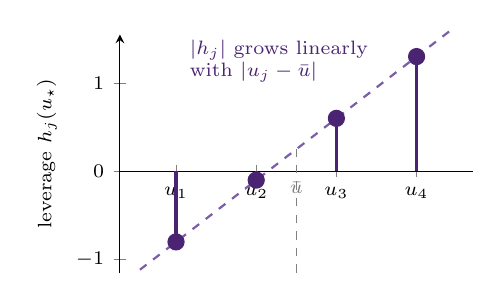
\begin{tikzpicture}
    \begin{axis}[
        clip=false, width=0.5\textwidth, height=0.38\textwidth,
        xmin=0.3, xmax=4.7, ymin=-1.15, ymax=1.55,
        axis x line=middle, axis y line=left,
        xtick={1,2,3,4}, xticklabels={$u_1$,$u_2$,$u_3$,$u_4$},
        ytick={-1,0,1}, tick label style={font=\scriptsize},
        ylabel={leverage $h_j(u_\star)$}, ylabel style={font=\scriptsize},
        x axis line style={-},
    ]
      \addplot[plummed, dashed, thick, domain=0.55:4.45, forget plot] {0.25+0.7*(x-2.5)};
      \addplot[ycomb, plumdark, very thick, mark=*, mark size=2.5pt]
          coordinates {(1,-0.80) (2,-0.10) (3,0.60) (4,1.30)};
      \draw[gray, dashed, thin] (axis cs:2.5,-1.15) -- (axis cs:2.5,0.25);
      \node[gray, font=\scriptsize, anchor=north] at (axis cs:2.5,-0.02) {$\bar u$};
      \node[plumdark, font=\scriptsize, anchor=west, align=left] at (axis cs:1.05,1.25)
          {$|h_j|$ grows linearly\\ with $|u_j-\bar u|$};
    \end{axis}
    \end{tikzpicture}
    \caption{
        Leverage of each measurement. The leverage $h_j(u_\star)$ (\Cref{eq:prediction-weights}) measures how strongly each measurement steers the extrapolated prediction. Its magnitude grows linearly with the distance $|u_j - \bar u|$ from the centroid, and its sign flips across $\bar u$, so the endpoints carry the most weight.
    }
    \label{fig:leverage}
    \vspace{-0.6cm}
\end{wrapfigure}


The weight $h_j(u_\star)$ is the sensitivity of the extrapolated prediction to the $j$-th measurement, we will refer to it as the \emph{leverage} of point $j$ \citep{hastie2009elements}. $|h_j(u_\star)|$ is large when $j$ is far from the center.
We illustrate this in \Cref{fig:leverage}.
Note that, because $u_\star$ lies outside the data range $|u_\star - \bar u|$ is large which is why extrapolated predictions are so sensitive to the measurements with the highest leverage.



\paragraph{Propagating errors.}
Suppose the measurement at scale $j$ is perturbed, $y_j \mapsto y_j + \epsilon$, while the others are exact. Because \Cref{eq:prediction-weights} is linear, the prediction shifts by exactly
%
\begin{equation}\label{eq:single-error}
    \delta \hat y(u_\star) = h_j(u_\star)\, \epsilon.
\end{equation}
%
As is standard for scaling laws, take the scales equally spaced in log space, $u_j = u_1 + (j - 1)\Delta$. Then $u_j - \bar u = (j - \bar\jmath)\Delta$ with center $\bar\jmath = \tfrac{K+1}{2}$, and $S_{uu} = \Delta^2 \sum_k (k - \bar\jmath)^2 = \Delta^2\, \tfrac{K(K^2 - 1)}{12}$. Extrapolating from the corrupted scale $j$ to a scale $i$ steps further, $u_\star = u_{j+i}$, the spacing $\Delta$ cancels and \Cref{eq:single-error} becomes
%
\begin{equation}\label{eq:propagation}
    \delta \hat y_{j+i} = \epsilon \left[\, \frac{1}{K} + \frac{12\, (j - \bar\jmath)(j + i - \bar\jmath)}{K(K^2 - 1)} \,\right].
\end{equation}
%
Note that, an error $\epsilon$ at scale $j$ shifts the extrapolated log-loss at scale $j + i$ by a factor that depends on how many scales $j$ is from the center $\bar\jmath$ and how far the extrapolation $i$ is. Errors at the endpoints of the fitting range are the most damaging, while an error at the center ($j = \bar\jmath$) contributes only the $\nicefrac{1}{K}$ intercept shift and is not amplified by extrapolation.

\begin{figure}[!hbt]
    \centering
    \definecolor{plumdark}{HTML}{4A2472}
    \definecolor{plummed}{HTML}{7B5EA7}
    \definecolor{plumlight}{HTML}{C4A0C8}
    \begin{tikzpicture}[>=stealth]
    \begin{axis}[
        name=bax,
        clip=false, scale only axis, width=0.8\textwidth, height=0.42\textwidth,
        xmin=-0.4, xmax=6.9, ymin=1.4, ymax=5.7,
        axis lines=left,
        xtick={1,2,3,4,6}, ytick={2,3,4,5},
        xticklabel=\empty, yticklabel=\empty,
        xmajorgrids=true, ymajorgrids=true,
        major grid style={draw=gray!20, very thin},
        major tick length=0pt,
        every axis plot/.append style={very thick},
        legend style={font=\scriptsize, draw=none, fill=none,
            at={(0.5,-0.62)}, anchor=north, legend columns=1, row sep=1pt},
        legend cell align=left,
    ]
      \addplot[draw=none, fill=plumlight, fill opacity=0.18, forget plot]
          coordinates {(4,1.4) (4,5.7) (6.9,5.7) (6.9,1.4)} \closedcycle;
      \node[font=\scriptsize, gray, anchor=north] at (axis cs:5.4,5.68) {extrapolation};
      \addplot[plumdark, domain=0:6.5] {5-0.5*x};
      \addlegendentry{true scaling law}
      \addplot[plumlight, dotted, line width=1.4pt, domain=0:6.5] {5.06-0.53*x};
      \addlegendentry{estimate with error at small-leverage scale, good fit}
      \addplot[plummed, dashed, domain=0:6.5] {4.7-0.32*x};
      \addlegendentry{estimate with error at large-leverage scale, bad fit}
      \addplot[only marks, mark=*, plumdark, mark size=2.2pt, forget plot]
          coordinates {(1,4.5) (2,4) (3,3.5) (4,3)};
      \addplot[only marks, mark=o, plummed, mark size=3pt, forget plot] coordinates {(4,3.6)};
      \draw[->, plummed, semithick, shorten <=1pt, shorten >=1pt] (axis cs:4,3.05) -- (axis cs:4,3.55);
      \node[plummed, font=\scriptsize, anchor=south west] at (axis cs:4.05,3.5) {$\epsilon$ far from center $u_4$};
      \draw[<->, plummed, semithick] (axis cs:6.15,2.02) -- (axis cs:6.15,2.78);
      \node[plummed, font=\scriptsize, anchor=west] at (axis cs:6.25,2.42)
          {$\delta\hat y = h_4\epsilon$};
      \addplot[only marks, mark=o, plumlight, mark size=3pt, forget plot] coordinates {(2,4.6)};
      \draw[->, plumlight, semithick, shorten <=1pt, shorten >=1pt] (axis cs:2,4.05) -- (axis cs:2,4.55);
      \node[font=\scriptsize, anchor=south, text=plumlight!80!black] at (axis cs:2,4.62)
          {$\epsilon$ near center $u_2$};
      \draw[<->, plumlight, semithick] (axis cs:5.85,1.9) -- (axis cs:5.85,2.02);
      \node[font=\scriptsize, anchor=east, text=plumlight!70!black] at (axis cs:5.75,1.75)
          {$\delta\hat y = h_2\epsilon$};
      \draw[gray, dashed, thin] (axis cs:2.5,1.4) -- (axis cs:2.5,3.75);
      \draw[gray, dashed, thin] (axis cs:6,1.4) -- (axis cs:6,3.0);
      \node[font=\scriptsize, anchor=north] at (axis cs:1,1.38) {$u_1$};
      \node[font=\scriptsize, anchor=north] at (axis cs:2,1.38) {$u_2$};
      \node[font=\scriptsize, anchor=north] at (axis cs:3,1.38) {$u_3$};
      \node[font=\scriptsize, anchor=north] at (axis cs:4,1.38) {$u_4$};
      \node[font=\scriptsize, anchor=north] at (axis cs:2.5,1.20) {$\bar u$};
      \node[font=\scriptsize, anchor=north] at (axis cs:6,1.38) {$u_\star$};
      \node[font=\small, anchor=west] at (axis cs:7.0,1.4) {$u=\log x$};
      \node[font=\small, anchor=south, rotate=90] at (axis cs:-0.4,5.2) {$y=\log L$};
    \end{axis}
    % second x-axis (below the first): centered index
    \begin{axis}[
        at={(bax.south west)}, anchor=north west, yshift=-22pt,
        clip=false, scale only axis, width=0.8\textwidth, height=1pt,
        xmin=-0.4, xmax=6.9, ymin=0, ymax=1,
        axis x line=bottom, hide y axis,
        xtick={1,2,3,4},
        xticklabels={$-\tfrac{3}{2}$,$-\tfrac{1}{2}$,$+\tfrac{1}{2}$,$+\tfrac{3}{2}$},
        x tick label style={font=\scriptsize, anchor=north},
    ]
      \node[font=\small, anchor=west] at (axis cs:7.0,0) {$j-\hat\jmath$};
    \end{axis}
    % third x-axis (below the second): leverage
    \begin{axis}[
        name=levax,
        at={(bax.south west)}, anchor=north west, yshift=-44pt,
        clip=false, scale only axis, width=0.8\textwidth, height=1pt,
        xmin=-0.4, xmax=6.9, ymin=0, ymax=1,
        axis x line=bottom, hide y axis,
        xtick={1,2,3,4},
        xticklabels={$-0.8$,$-0.1$,$+0.6$,$+1.3$},
        x tick label style={font=\scriptsize, anchor=north},
    ]
      \node[font=\small, anchor=west] at (axis cs:7.0,0) {$h_j(u_\star)$};
    \end{axis}
    % extend the left (y) axis down so it meets the bottom-most x-axis
    \draw[thin] (bax.south west) -- (levax.south west);
    \end{tikzpicture}
    \caption{
        Consequence for extrapolation. Losses are measured at $K$ equally spaced scales $u_1, \dots, u_K$ (centroid $\bar u$) and fit by ordinary least squares (solid; \Cref{eq:loglog} and \ref{eq:ols-slope}). Perturbing a measurement by the same $\epsilon$ shifts the extrapolated prediction at $u_\star$ by $\delta\hat y = h_j(u_\star)\,\epsilon$ (\Cref{eq:single-error}): a high-leverage point far from the center ($u_4$, dashed) \emph{amplifies} the error, while a low-leverage point near the center ($u_2$, dotted) barely moves it. Because $u_\star$ lies far outside the data range (shaded), it amplifies the effect of the leverage further ($h_4(u_\star) > 1$ here). The lower axes read each measurement's centered index $j-\hat\jmath$ and its leverage $h_j(u_\star)$.
    }
    \label{fig:scaling-error-propagation}
\end{figure}

\subsection{How many hyperparameter runs are needed?}
\label{app:background:how-close-does-random-search-get}

How many hyperparameter runs are needed to approximate the optimal perplexity at a given scale? Or in other words, how quickly does the sample minimum of the noisy quadratic converge to the best attainable performance $\alpha$? We will see that the answer depends on the intrinsic dimension $\gamma$ of the hyperparameter space.

Given the noisy quadratic limit (see \Cref{app:background:the-noisy-quadratic-limit}), whose notation ($\alpha$, $\beta$, $\gamma$, $\sigma$, and the CDF $F$) we adopt throughout, we can quantify how close random search gets to the best attainable performance $\alpha$ after $M$ evaluations, i.e. how many hyperparameter runs get us a good estimate for the best attainable performance at a given scale. Let $Y_1, \dots, Y_M$ be i.i.d.\ scores drawn within the asymptotic regime so each $Y_i$ follows the noisy quadratic distribution of \Cref{eq:noisy-quadratic-limit}, and let $T_M = \min_{i \leq M} Y_i$ be the best score found.

First, we find the CDF of $T_M$, by reasoning about the complement: the best score exceeds a threshold $y$ only when \emph{every} draw does, and a single draw exceeds $y$ with probability $\Prob(Y_i > y) = 1 - F(y)$, and because we draw independent samples,
%
\begin{equation}\label{eq:min-survival}
    \Prob(T_M > y) = \prod_{i=1}^{M} \Prob(Y_i > y) = \prod_{i=1}^{M} \underbrace{\bigl(1 - F(y)\bigr)}_{=\,\Prob(Y_i > y)} = \bigl(1 - F(y)\bigr)^M.
\end{equation}
%
Taking the complement gives the CDF of the minimum $T_M$,
%
\begin{equation}\label{eq:min-cdf}
    \Prob(T_M \leq y) = 1 - \bigl(1 - F(y)\bigr)^M.
\end{equation}


Second, we determine how $T_M$ approaches the optimum $\alpha$ as $M$ grows by consulting Extreme Value Theory (EVT)\citep{gnedenko1943distribution, de2006extreme}
\footnote{
    Extreme-value theory is usually stated for maxima; the result for minima follows by applying it to $-Y$.
}.
We will see there are two regimes: the noiseless case ($\sigma = 0$) and the noisy case ($\sigma > 0$) for which we will come to different conclusions.
Consider the noiseless case ($\sigma = 0$), where $\alpha$ is the lower endpoint of the support and the tail is the power law of \Cref{eq:quadratic-cdf}. A distribution with a finite endpoint and a polynomially decaying tail lies in the \emph{Weibull domain of attraction} of EVT: its sample minima, once recentered at the endpoint and rescaled, converge to a Weibull law. Concretely, take the natural scale $a_M := (\beta - \alpha)\, M^{-2/\gamma}$, defined implicitly by $F(\alpha + a_M) = 1/M$. Substituting $u = a_M t$ yields $\bigl(1 - F(\alpha + a_M t)\bigr)^M \to \exp(-t^{\gamma/2})$, so the rescaled gap converges in distribution to 

%
\begin{equation}\label{eq:sample-min-weibull}
    \frac{T_M - \alpha}{a_M} \;\xrightarrow{\;d\;}\; \operatorname{Weibull}(k), \qquad k = \tfrac{\gamma}{2},
\end{equation}
%
where $\operatorname{Weibull}(k)$ is the Weibull distribution of shape $k$ and unit scale, see \Cref{fig:weibull-shapes} for an illustration.
%
\begin{figure}[!hbt]
    \centering
    \definecolor{plumdark}{HTML}{4A2472}
    \definecolor{plummed}{HTML}{7B5EA7}
    \definecolor{plumlight}{HTML}{C4A0C8}
    \begin{tikzpicture}
        \begin{axis}[
            clip=false,
            width=0.6\textwidth, height=0.36\textwidth,
            domain=0.05:4, samples=200,
            ymin=0, ymax=1.5, xmin=0,
            axis lines=left,
            xlabel={rescaled gap $x = (T_M - \alpha)/a_M$},
            ylabel={density},
            xlabel style={font=\scriptsize}, ylabel style={font=\scriptsize},
            tick label style={font=\scriptsize},
            legend style={font=\scriptsize, draw=none, fill=none, at={(0.03,0.97)}, anchor=north west},
            every axis plot/.append style={very thick},
        ]
            \addplot[draw=none, fill=plummed, fill opacity=0.13, forget plot]
                coordinates {(2.5,0) (2.5,1.5) (4,1.5) (4,0)} \closedcycle;
            \addplot[plumlight, domain=0.08:4] {0.5*x^(-0.5)*exp(-(x^0.5))};
            \addlegendentry{$\gamma=1\ (k=\tfrac12)$}
            \addplot[plummed]   {exp(-x)};
            \addlegendentry{$\gamma=2\ (k=1)$}
            \addplot[plumdark]  {1.5*(x^0.5)*exp(-(x^1.5))};
            \addlegendentry{$\gamma=3\ (k=\tfrac32)$}
            \node[font=\scriptsize, plumdark, align=center] at (axis cs:3.25,0.75)
                {upper tail\\[-1pt] $\lesssim e^{-x^{k}}$};
            \addplot[only marks, mark=*, plumdark, mark size=2pt, forget plot]
                coordinates {(0,0)};
            \draw[->, plumdark, thin] (axis cs:-0.55,0.3) -- (axis cs:-0.02,0.02);
            \node[font=\scriptsize, plumdark, anchor=east] at (axis cs:-0.6,0.34)
                {endpoint $\alpha$};
        \end{axis}
    \end{tikzpicture}
    \caption{
        Weibull($k$) densities $f(x) = k\, x^{k-1} e^{-x^{k}}$ (and CDF $F(x) = 1 - e^{-x^{k}}$).  The shape $k = \gamma/2$ governs how quickly probability accumulates away from the endpoint $\alpha$: a small effective dimension ($\gamma = 1$) piles mass near the optimum, while larger $\gamma$ pushes the typical gap outward. In the shaded \emph{upper tail} every density decays at least as fast as $e^{-x^{k}}$, so a vanishing fraction of both the mass and the mean sits out there, which illustrates why this function is uniformly integrable, meaning that the mean exists.
    }
    \label{fig:weibull-shapes}
\end{figure}

Third, as the limit in \Cref{eq:sample-min-weibull} is a convergence in distribution, it does not by itself imply convergence of its mean $E[(T_M-\alpha)/a_M]$. For this, we have to additionally show that the rescaled minimum is \emph{uniformly integrable}, which ensures that the mean exists. To see this condition is fulfilled, note that the upper tail is bounded by $\exp(-t^{\gamma/2})$.
Thus, the rescaled minimum is uniformly integrable and the mean converges to that of the limiting Weibull distribution;
\begin{equation}\label{eq:sample-min-rescaled-mean}
    \E\!\left[\frac{T_M - \alpha}{a_M}\right] \;\longrightarrow\; \E\bigl[\operatorname{Weibull}(k)\bigr] = \Gamma\!\left(1 + \tfrac{1}{k}\right),
\end{equation}
 where $\Gamma$ is the gamma function \citep{johnson1994continuous}.


Finally, we have all the pieces to show how quickly the gap between the observed and optimal minima, $\E[T_M] - \alpha$, closes as the number of samples $M$ increases. Its dependence on $M$ follows from \Cref{eq:sample-min-weibull} by multiplying through by the scale $a_M = (\beta - \alpha)\, M^{-2/\gamma}$ and setting $k = \gamma/2$,
%
\begin{equation}\label{eq:sample-min-mean}
    \E[T_M] - \alpha \;\sim\;
    a_M \, \Gamma\!\left(1 + \tfrac{1}{k}\right) \;=\; \underbrace{(\beta - \alpha)\, \Gamma\!\left(1 + \tfrac{2}{\gamma}\right)}_{=: C(\gamma)} \; M^{-2/\gamma}.
\end{equation}

Here and below, $\sim$ denotes \emph{asymptotic equivalence}: $f(M) \sim g(M)$ means $f(M)/g(M) \to 1$ as $M \to \infty$, not proportionality or ``distributed as''. For the practically relevant cases $\gamma \in \{1, 2\}$ the mean can even be evaluated exactly,\footnote{
    The ``$\sim$'' in \Cref{eq:sample-min-mean} is asymptotic: it is the $M \to \infty$ limit of the Weibull law \Cref{eq:sample-min-weibull}, whose mean is the standard $\Gamma(1 + 1/k)$. For the noiseless quadratic we can go further and evaluate the mean exactly at finite $M$. Using the tail identity $\E[Z] = \int_0^\infty \Prob(Z > u)\, \d u$ for the nonnegative $Z = T_M - \alpha$ together with the survival function \Cref{eq:min-survival}, the gap is a Beta integral,
    %
    \begin{equation}\label{eq:sample-min-exact}
        \E[T_M] - \alpha
        = \int_0^{\beta - \alpha} \bigl(1 - F(\alpha + u)\bigr)^M\, \d u
        = (\beta - \alpha)\, \Gamma\!\left(1 + \tfrac{2}{\gamma}\right) \frac{\Gamma(M + 1)}{\Gamma\!\left(M + 1 + \nicefrac{2}{\gamma}\right)}.
    \end{equation}
    %
    The ratio of the two gamma functions decays like $M^{-2/\gamma}$ as $M \to \infty$, recovering \Cref{eq:sample-min-mean}. Since the number of runs $M$ is an integer, $\Gamma(M + 1) = M!$, and whenever $2/\gamma$ is a positive integer the ratio collapses to a rational function of $M$, giving the exact expressions in \Cref{eq:sample-min-mean-exact}.
}
giving the main result of this section:
%
%\begin{tcolorbox}[colback=plumbox, colframe=plumdark, boxrule=0.8pt, arc=2pt,
    left=8pt, right=8pt, top=4pt, bottom=4pt]
\begin{equation}\label{eq:sample-min-mean-exact}
    \E[T_M] - \alpha \;
    \begin{cases}
         \sim\; C(\gamma)\, M^{-2/\gamma}, & \text{for all } \gamma,\\[1.6ex]
        = \dfrac{2(\beta - \alpha)}{(M+1)(M+2)} \;\sim\; 2(\beta - \alpha)\, M^{-2}, & \text{for } \gamma = 1,\\[1.6ex]
        = \dfrac{\beta - \alpha}{M+1} \;\sim\; (\beta - \alpha)\, M^{-1}, & \text{for } \gamma = 2.
    \end{cases}
\end{equation}
%\end{tcolorbox}

Thus the best score approaches $\alpha$ as a power law in the number of evaluations, $M^{-2/\gamma}$, with the exponent set by the effective number of hyperparameters. Each additional effective hyperparameter flattens the convergence exponent.

As a concrete example, say we ran 100 hyperparameter evaluations at a scale where $\gamma = 2$. Assuming all other scales have the same $\alpha$ and $\beta$, we can compare how many runs would be needed at other scales where $\gamma = 1, 3$ to reach the same quality, i.e.\ the same gap.
Matching the gaps in \Cref{eq:sample-min-mean-exact}, i.e.\ $C(\gamma)\, M_\gamma^{-2/\gamma} = C(2)\, 100^{-1}$, gives $M_\gamma = \bigl[\,100\, C(\gamma)/C(2)\,\bigr]^{\gamma/2}$. Since $C(1) = 2(\beta - \alpha)$, $C(2) = (\beta - \alpha)$, and $C(3) \approx 0.903\,(\beta - \alpha)$, the constant ratios are $C(1)/C(2) = 2$ and $C(3)/C(2) \approx 0.903$, so
%
\begin{equation*}
    M_1 = (100 \cdot 2)^{1/2}  \approx 14
    \quad\text{and}\quad
    M_3 = (100 \cdot 0.903)^{3/2}  \approx 858.
\end{equation*}
%
So dropping from two effective hyperparameters to one cuts the tuning cost from $100$ runs to about $14$ (a $7\times$ saving), while adding one raises it to nearly $900$ (a further $8.6\times$).

Note that we assumed $\sigma = 0$ for our derivation, when $\sigma > 0$, the unbounded Gaussian tail means we can no longer rely on the same analysis as the EVT is now in the heavy tail regime.




\subsection{Compute-optimal tuning across scales}
\label{sec:compute-optimal-tuning}

In this section we will combine the results from the previous two sections to answer the question: Given a fixed compute budget, how should we split it across scales to minimize the error at the scale we extrapolate to?

For our analysis, we make the following assumptions, 
%
\begin{enumerate}[noitemsep]
    \item \textbf{Tuning error per scale.} At scale $j$ we run random search with $M_j$ configurations and record the best. Its expected gap to the optimum is $\epsilon_j = A_j\, M_j^{-2/\gamma_j}$ with $A_j = (\beta_j - \alpha_j)\,\Gamma(1 + 2/\gamma_j)$ (\Cref{eq:sample-min-mean}), where $\gamma_j$ is the effective number of hyperparameters at that scale.
    \item \textbf{Cost.} Compute per run scales linearly with the parameter count, so one run at scale $j$ costs $\propto N_j$. The scales are geometric, $N_j = N_1 \rho^{\,j-1}$ (equidistant in $\log N$), and the total budget is $C = \sum_{j=1}^{K} M_j N_j$.
    \item \textbf{Propagation.} An error $\epsilon_j$ shifts the extrapolated prediction by $h_j\,\epsilon_j$ (\Cref{eq:single-error}), where $h_j = h_j(u_\star)$ is the leverage of scale $j$ at the target $u_\star$. We minimize the propagated-error bound $E_\star = \sum_{j} |h_j|\, \epsilon_j$.\footnote{
        Using the triangle inequality on $\sum_j h_j \epsilon_j$ gives a sign-robust objective. Minimizing the variance proxy $\sum_j h_j^2 \epsilon_j^2$ instead replaces the exponent $\nicefrac{\gamma_j}{(\gamma_j + 2)}$ below by $\nicefrac{\gamma_j}{(\gamma_j + 4)}$ and leaves the qualitative allocation unchanged.
    }
    \item \textbf{Effective dimension.} Empirically $\gamma_j \in \{1, 2\}$, and it \emph{decreases} with scale: the low-compute scales have $\gamma_j = 2$, and beyond some scale the effective dimension drops to $\gamma_j = 1$.
\end{enumerate}

\paragraph{The optimization problem.}
Substituting the tuning error $\epsilon_j = A_j M_j^{-2/\gamma_j}$ into the propagated-error bound, the quantity we want to minimize with respect to the number of runs $M_j$ is
%
\begin{equation}\label{eq:objective}
    E_\star(M_1, \dots, M_K) = \sum_{j=1}^{K} |h_j|\, \epsilon_j = \sum_{j=1}^{K} |h_j|\, A_j\, M_j^{-2/\gamma_j},
\end{equation}
%
however this error minimization is subject to the compute budget constraint \Cref{eq:constraint};
%
\begin{equation}\label{eq:constraint}
    \sum_{j=1}^{K} M_j N_j = C.
\end{equation}
%
We attach the constraint with a Lagrangian multiplier $\lambda$ and minimize the loss
%
\begin{equation}\label{eq:lagrangian}
    \mathcal{L}(M_1, \dots, M_K, \lambda) = \sum_{j=1}^{K} |h_j|\, A_j\, M_j^{-2/\gamma_j} + \lambda\left(\sum_{j=1}^{K} M_j N_j - C\right).
\end{equation}
%
Differentiating with respect to a single $M_j$ gives ,
%
\begin{equation}\label{eq:foc}
    \frac{\partial \mathcal{L}}{\partial M_j}
    = -\frac{2}{\gamma_j}\, |h_j|\, A_j\, M_j^{-2/\gamma_j - 1} + \lambda N_j
    = 0.
\end{equation}
%
Rearranged for $\lambda$;
%
\begin{equation}\label{eq:equimarginal}
    \underbrace{\frac{1}{N_j}\cdot\frac{2}{\gamma_j}\, |h_j|\, A_j\, M_j^{-2/\gamma_j - 1}}_{\text{error reduction per unit compute at scale } j} = \lambda \quad\text{for every active scale } j.
\end{equation}
%
Solve for $M_j$ in \Cref{eq:foc},
%
\begin{equation}\label{eq:solve-step}
    M_j^{2/\gamma_j + 1} = \frac{2\, |h_j|\, A_j}{\gamma_j\, \lambda\, N_j}.
\end{equation}
%
The exponent on the left combines as $\dfrac{2}{\gamma_j} + 1 = \dfrac{\gamma_j + 2}{\gamma_j}$, so raising both sides to the reciprocal power $\dfrac{\gamma_j}{\gamma_j + 2}$ gives the optimal number of runs,
%
\begin{equation}\label{eq:opt-runs}
    M_j^\star = \left(\frac{2\,|h_j|\, A_j}{\gamma_j\, \lambda\, N_j}\right)^{\frac{\gamma_j}{\gamma_j + 2}}
    \;\propto\; \left(\frac{|h_j|}{\gamma_j\, N_j}\right)^{\frac{\gamma_j}{\gamma_j + 2}}.
\end{equation}
%
\paragraph{Example.}
To make the allocation concrete, take $K = 4$ equally spaced scales and extrapolate one step beyond the fitted range, $u_\star = u_{K+1}$ (i.e.\ $i = 1$ in \Cref{eq:propagation}). With centre $\bar\jmath = \tfrac{K+1}{2} = \tfrac52$, the target sits at $u_\star - \bar u = \bar\jmath\,\Delta$ and the index form of the leverage collapses to a single line,
%
\begin{equation}\label{eq:example-leverage}
    h_j = \frac{1}{K} + \frac{12\,\bar\jmath\,(j - \bar\jmath)}{K(K^2 - 1)}
        = \frac{j - 2}{2},
    \qquad\text{so}\qquad
    \bigl(|h_1|, |h_2|, |h_3|, |h_4|\bigr) = \left(\tfrac12,\; 0,\; \tfrac12,\; 1\right).
\end{equation}
%
The endpoint nearest the target ($j = 4$) carries the most leverage, while the near-central scale ($j = 2$) carries essentially none. Following the fourth assumption, the effective dimension drops across the centroid: $\gamma_j = 2$ for the small scales below the centre ($j = 1, 2$) and $\gamma_j = 1$ for the large scales above it ($j = 3, 4$). The per-run costs are geometric in the index, $N_j = N_1\, \rho^{\,j-1}$, i.e.\ linear in log space, $\log N_j = \log N_1 + (j-1)\log\rho$.

Substituting into \Cref{eq:opt-runs} and reading off the exponent $\tfrac{\gamma_j}{\gamma_j + 2}$ ($= \tfrac12$ where $\gamma_j = 2$, $= \tfrac13$ where $\gamma_j = 1$), the optimal number of runs at each scale is
%
\begin{equation}\label{eq:example-runs}
    M_j^\star \;\propto\; \left(\frac{|h_j|}{\gamma_j\, N_j}\right)^{\frac{\gamma_j}{\gamma_j + 2}}
    = \begin{cases}
        \bigl(\,|h_j| / (2\, N_1 \rho^{\,j-1})\,\bigr)^{1/2}, & j \le 2 \quad (\gamma_j = 2),\\[6pt]
        \bigl(\,|h_j| / (N_1 \rho^{\,j-1})\,\bigr)^{1/3}, & j \ge 3 \quad (\gamma_j = 1).
    \end{cases}
\end{equation}
%
Multiplying by $N_j$ gives the compute placed at each scale,
%
\begin{equation}\label{eq:opt-compute}
    C_j^\star = N_j\, M_j^\star \;\propto\; \left(\frac{|h_j|}{\gamma_j}\right)^{\frac{\gamma_j}{\gamma_j + 2}} N_j^{\frac{2}{\gamma_j + 2}},
\end{equation}
%
whose exponent on $N_j$ ($\tfrac12$ then $\tfrac23$) is below one, so compute grows \emph{sublinearly} with a scale's per-run cost. Within the large-scale regime the two upper scales are tied together cleanly,
%
\begin{equation}\label{eq:example-ratio}
    \frac{M_4^\star}{M_3^\star} = \left(\frac{|h_4|}{|h_3|}\cdot\frac{N_3}{N_4}\right)^{1/3} = \left(\frac{2}{\rho}\right)^{1/3},
    \qquad
    \frac{C_4^\star}{C_3^\star} = 2^{1/3}\,\rho^{2/3}.
\end{equation}
%
For any $\rho > 2$ the larger scale receives \emph{fewer} runs yet \emph{more} compute than its neighbour: a handful of expensive runs at the top outweighs many cheap ones below. \Cref{fig:compute-allocation} plots the allocation for $\rho = 4$ ($N_j = 1, 4, 16, 64$): the number of runs is largest at the cheap bottom scale and tapers off, while the compute share climbs monotonically and piles up at the top scale. The near-central scale $j = 2$, with $h_2 \approx 0$, drops out entirely and is kept only by its single anchoring run.

\begin{figure}[!htb]
    \centering
    \definecolor{plumdark}{HTML}{4A2472}
    \definecolor{plummed}{HTML}{7B5EA7}
    \definecolor{plumlight}{HTML}{C4A0C8}
    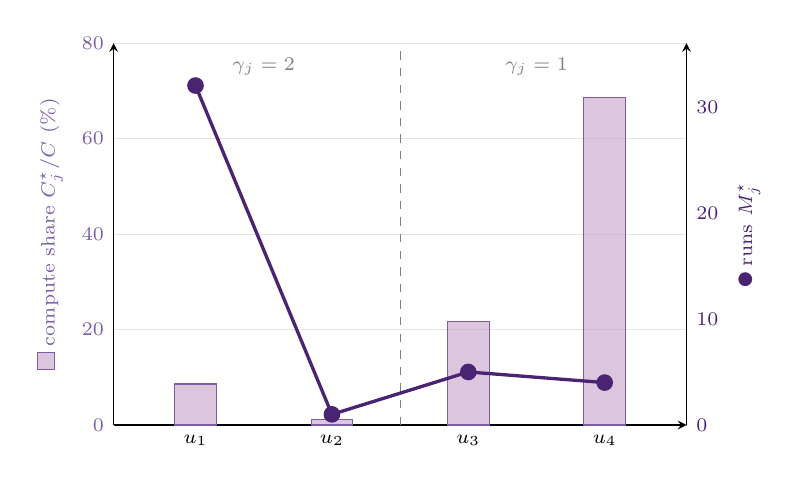
\begin{tikzpicture}
    \begin{axis}[
        name=cax,
        clip=false, scale only axis, width=0.6\textwidth, height=0.4\textwidth,
        xmin=0.4, xmax=4.6, ymin=0, ymax=80,
        axis y line=left, axis x line=bottom,
        xtick={1,2,3,4}, xticklabels={$u_1$,$u_2$,$u_3$,$u_4$},
        ytick={0,20,40,60,80},
        tick label style={font=\scriptsize},
        ylabel={\tikz{\draw[draw=plummed, fill=plumlight, fill opacity=0.6] (0,0) rectangle (6pt,6pt);}\;compute share $C_j^\star/C$ (\%)},
        ylabel style={font=\scriptsize, text=plummed},
        y tick label style={text=plummed},
        major tick length=0pt,
        ymajorgrids=true, major grid style={draw=gray!20, very thin},
    ]
      \addplot[ybar, bar width=15pt, draw=plummed, fill=plumlight, fill opacity=0.6]
          coordinates {(1,8.6) (2,1.1) (3,21.6) (4,68.7)};
      \draw[gray, dashed, thin] (axis cs:2.5,0) -- (axis cs:2.5,80);
      \node[gray, font=\scriptsize, anchor=north] at (axis cs:1.5,79) {$\gamma_j = 2$};
      \node[gray, font=\scriptsize, anchor=north] at (axis cs:3.5,79) {$\gamma_j = 1$};
    \end{axis}
    \begin{axis}[
        at={(cax.south west)}, anchor=south west,
        clip=false, scale only axis, width=0.6\textwidth, height=0.4\textwidth,
        xmin=0.4, xmax=4.6, ymin=0, ymax=36,
        axis y line=right, axis x line=none, xtick=\empty,
        ytick={0,10,20,30},
        tick label style={font=\scriptsize},
        ylabel={\tikz{\node[circle, fill=plumdark, inner sep=0pt, minimum size=5pt]{};}\;runs $M_j^\star$},
        ylabel style={font=\scriptsize, text=plumdark},
        y tick label style={text=plumdark},
        major tick length=0pt,
    ]
      \addplot[plumdark, very thick, mark=*, mark size=2.4pt]
          coordinates {(1,32) (2,1) (3,5) (4,4)};
    \end{axis}
    \end{tikzpicture}
    \caption{
        Compute-optimal allocation across $K = 4$ scales for the example of \Cref{eq:example-leverage} and \ref{eq:example-runs} ($\rho = 4$, extrapolating one step past the range). Bars (left axis) show the share of the budget spent at each scale $C_j^\star / C$; the line (right axis) shows the number of runs $M_j^\star$. Cheap low scales absorb many runs but little compute; the budget concentrates on the high-leverage, low-$\gamma$ scale nearest the target ($u_4$), which is bought with only a few expensive runs. The near-central scale $u_2$ has $h_2 \approx 0$ and is kept only to anchor the fit.
    }
    \label{fig:compute-allocation}
\end{figure}

\paragraph{A manual for designing a compute-optimal scaling law estimate.}

Any practitioner should roughly follow the following steps in designing their experiment:

\begin{enumerate}
    \item  \emph{Estimate (or set) $\rho$}, the relative cost of a scale $N_j = N_1\,\rho^{\,j-1}$. For transformers this cost is well approximated by the standard $6ND$ estimate (roughly six FLOPs per parameter per token over the forward and backward pass) \citep{Kaplan2020ScalingLaws, Hoffmann2022AnEmpirical}, so once a practitioner chooses a model ladder and its token counts, every $N_j$, and hence $\rho$, is fixed. (Anyone building their own ladder has to do this FLOP accounting up front to know what a run at each scale will cost.) 
    \item \emph{Assume the effective dimensions $\gamma_j$.} We take these as known. This is not a perfect assumption, but it is broadly understood where along a model ladder tuning becomes reliable and $\gamma$ drops, and the choice can be checked after the fact from the realized slope of error against compute at each scale. 
    \item \emph{Compute the total budget $C$.} This is normally known outright usually in GPU-hours, converted to FLOPs through the hardware's sustained throughput. The only remaining factor, the per-scale error amplitude $A_j$, varies slowly and is typically taken comparable across scales (or read off the loss spread if not).
\end{enumerate}


With $\rho$, the $\gamma_j$, and $C$ in hand, the number of runs per scale can be computed. The multiplier $\lambda$ is computed through \Cref{eq:opt-runs}, and it is set by substituting the $M_j^\star$ into the budget constraint $\sum_j M_j N_j = C$ (\Cref{eq:constraint}) and solving the resulting equation for $\lambda$. Reading the $M_j^\star$ back out of \Cref{eq:opt-runs} then gives the number of tuning runs to launch at each scale.




